\documentclass{standalone}
\usepackage{tikz}
\usetikzlibrary{patterns, positioning}
\usepackage[sfdefault]{ClearSans} %% option 'sfdefault' activates Clear Sans as the default text font
\usepackage[T1]{fontenc}

\begin{document}
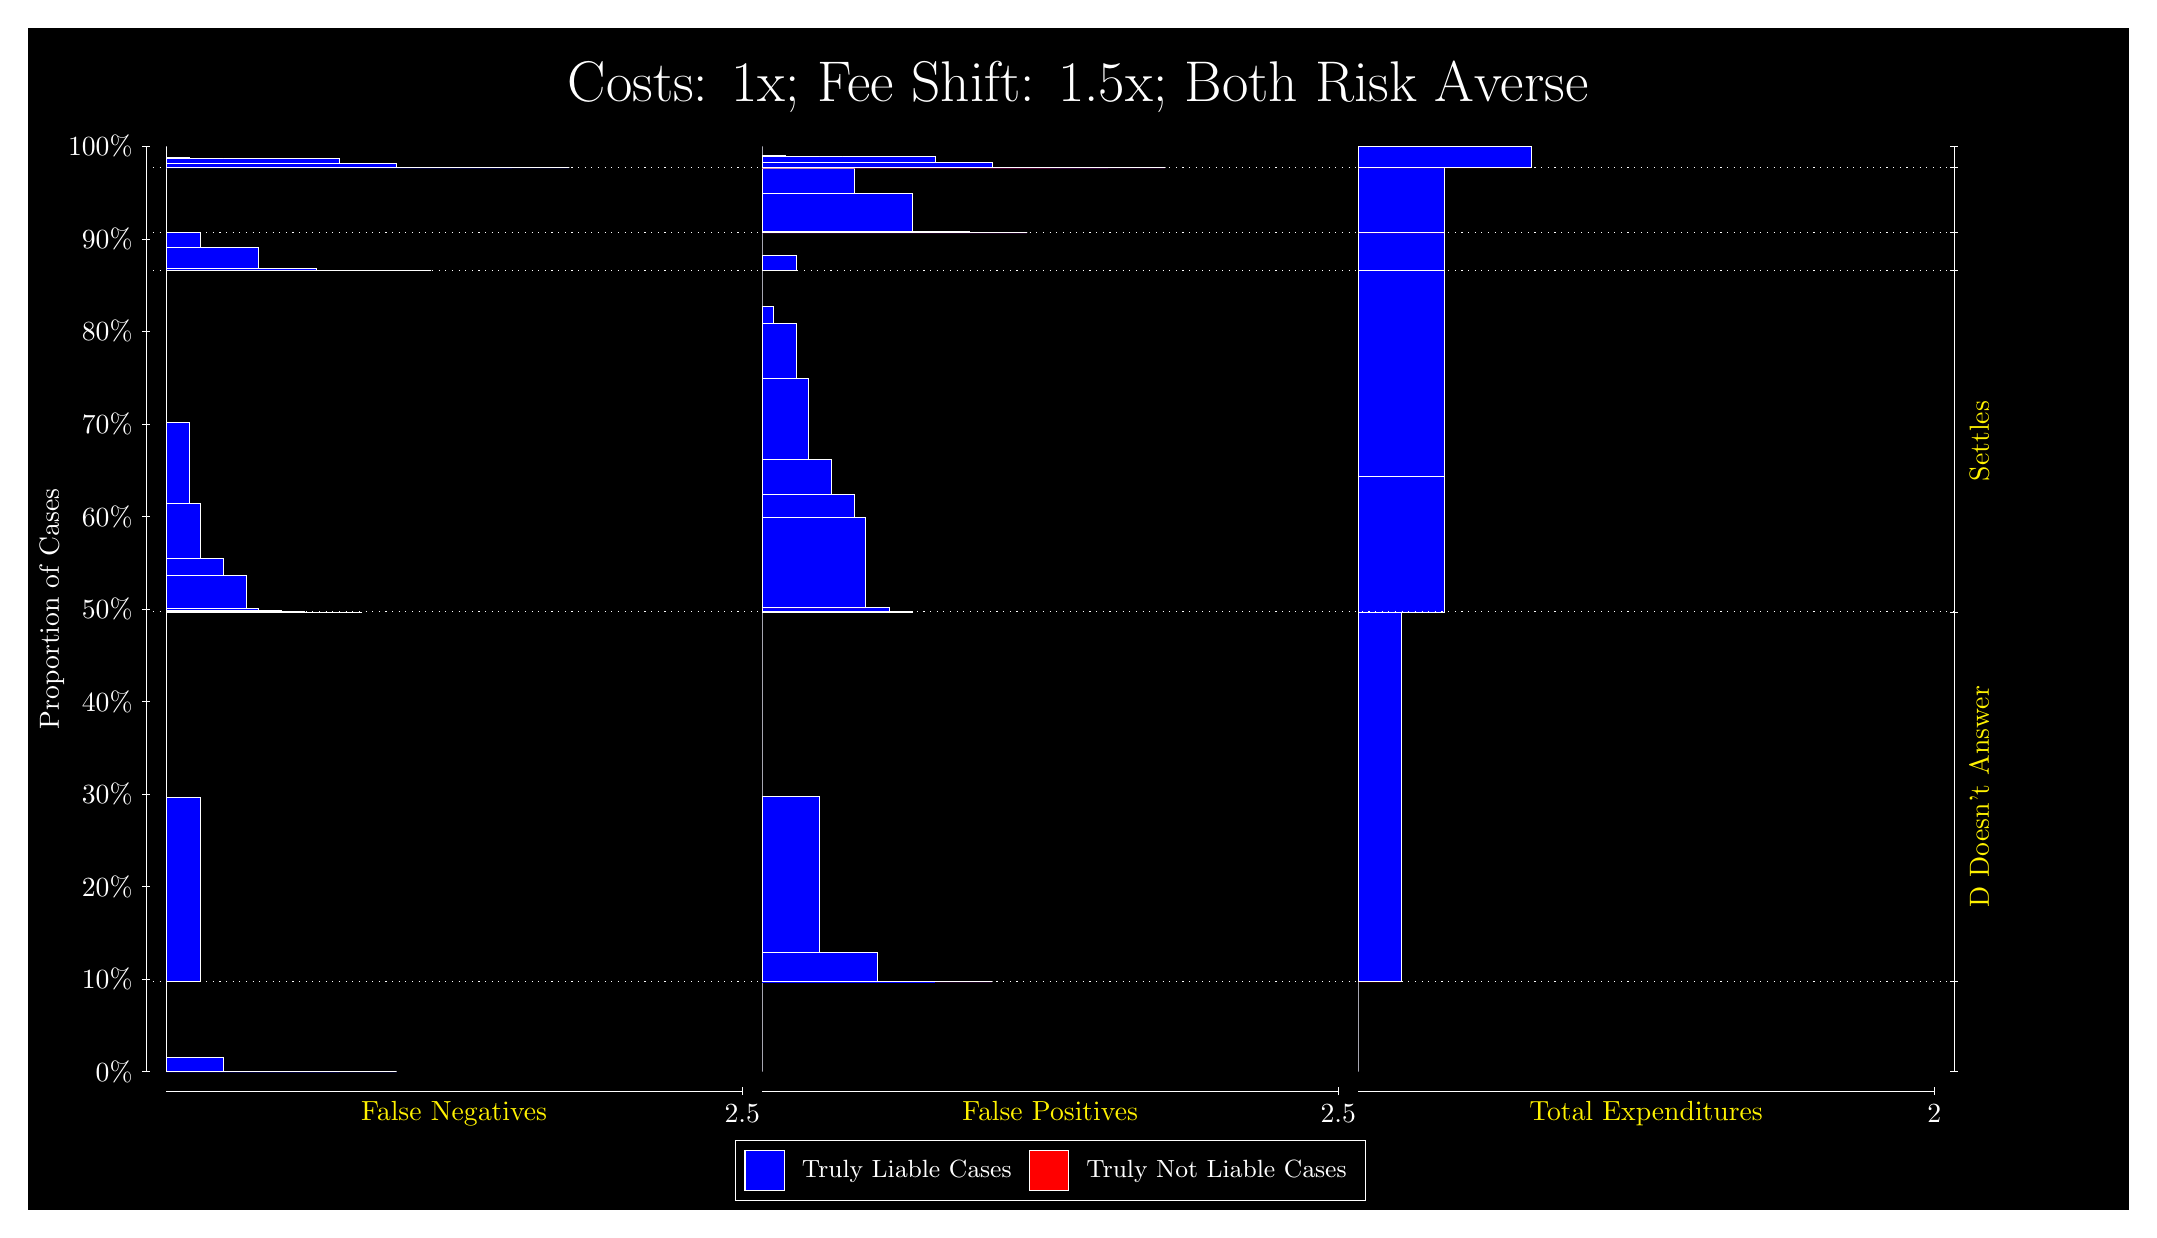
\begin{tikzpicture}
\draw[fill=black] (0,0) rectangle (26.667,15);
\draw[text=white] (0,13.5) rectangle (26.667,15) node[midway] {\huge Costs: 1x; Fee Shift: 1.5x; Both Risk Averse};
\draw[white, very thin] (1.5,1.75) -- (1.5,13.5);
\node[rotate=90, text=white, anchor=center] at (0.3, 7.625) {Proportion of Cases};
\draw[white, very thin] (1.45,1.75) -- (1.55,1.75);
\node[text=white, anchor=east] at (1.45, 1.75) {0\%};
\draw[white, very thin] (1.45,2.925) -- (1.55,2.925);
\node[text=white, anchor=east] at (1.45, 2.925) {10\%};
\draw[white, very thin] (1.45,4.1) -- (1.55,4.1);
\node[text=white, anchor=east] at (1.45, 4.1) {20\%};
\draw[white, very thin] (1.45,5.275) -- (1.55,5.275);
\node[text=white, anchor=east] at (1.45, 5.275) {30\%};
\draw[white, very thin] (1.45,6.45) -- (1.55,6.45);
\node[text=white, anchor=east] at (1.45, 6.45) {40\%};
\draw[white, very thin] (1.45,7.625) -- (1.55,7.625);
\node[text=white, anchor=east] at (1.45, 7.625) {50\%};
\draw[white, very thin] (1.45,8.8) -- (1.55,8.8);
\node[text=white, anchor=east] at (1.45, 8.8) {60\%};
\draw[white, very thin] (1.45,9.975) -- (1.55,9.975);
\node[text=white, anchor=east] at (1.45, 9.975) {70\%};
\draw[white, very thin] (1.45,11.15) -- (1.55,11.15);
\node[text=white, anchor=east] at (1.45, 11.15) {80\%};
\draw[white, very thin] (1.45,12.325) -- (1.55,12.325);
\node[text=white, anchor=east] at (1.45, 12.325) {90\%};
\draw[white, very thin] (1.45,13.5) -- (1.55,13.5);
\node[text=white, anchor=east] at (1.45, 13.5) {100\%};

\draw[white, very thin] (24.457,1.75) -- (24.457,13.5);
\draw[white, very thin] (24.407,1.75) -- (24.507,1.75);
\node[anchor=west] at (24.407, 1.75) {};
\draw[white, very thin] (24.407,2.8901) -- (24.507,2.8901);
\node[anchor=west] at (24.407, 2.8901) {};
\draw[white, very thin] (24.407,7.5885) -- (24.507,7.5885);
\node[anchor=west] at (24.407, 7.5885) {};
\draw[white, very thin] (24.407,11.927) -- (24.507,11.927);
\node[anchor=west] at (24.407, 11.927) {};
\draw[white, very thin] (24.407,12.405) -- (24.507,12.405);
\node[anchor=west] at (24.407, 12.405) {};
\draw[white, very thin] (24.407,13.229) -- (24.507,13.229);
\node[anchor=west] at (24.407, 13.229) {};
\draw[white, very thin] (24.407,13.5) -- (24.507,13.5);
\node[anchor=west] at (24.407, 13.5) {};

\draw[white, very thin, fill=blue] (1.75,1.75) rectangle (4.6775,1.75);
\draw[white, very thin, fill=blue] (1.75,1.75) rectangle (3.9457,1.75);
\draw[white, very thin, fill=blue] (1.75,1.75) rectangle (3.2138,1.7516);
\draw[white, very thin, fill=blue] (1.75,1.7516) rectangle (2.4819,1.9367);
\draw[white, very thin, fill=red] (1.75,1.9367) rectangle (1.75,1.9367);
\draw[white, very thin, fill=blue] (1.75,1.9367) rectangle (1.75,2.8901);
\draw[white, very thin, fill=blue] (1.75,2.8901) rectangle (2.1891,5.2363);
\draw[white, very thin, fill=red] (1.75,5.2363) rectangle (1.75,5.2363);
\draw[white, very thin, fill=blue] (1.75,5.2363) rectangle (1.75,7.5885);
\draw[white, very thin, fill=blue] (1.75,7.5885) rectangle (4.2384,7.5885);
\draw[white, very thin, fill=blue] (1.75,7.5885) rectangle (3.9457,7.5885);
\draw[white, very thin, fill=blue] (1.75,7.5885) rectangle (3.6529,7.5885);
\draw[white, very thin, fill=blue] (1.75,7.5885) rectangle (3.5065,7.6009);
\draw[white, very thin, fill=blue] (1.75,7.6009) rectangle (3.2138,7.6053);
\draw[white, very thin, fill=blue] (1.75,7.6053) rectangle (2.921,7.6354);
\draw[white, very thin, fill=blue] (1.75,7.6354) rectangle (2.7746,8.0517);
\draw[white, very thin, fill=blue] (1.75,8.0517) rectangle (2.4819,8.2669);
\draw[white, very thin, fill=blue] (1.75,8.2669) rectangle (2.1891,8.9618);
\draw[white, very thin, fill=blue] (1.75,8.9618) rectangle (2.0428,9.9935);
\draw[white, very thin, fill=red] (1.75,9.9935) rectangle (1.75,9.9935);
\draw[white, very thin, fill=blue] (1.75,9.9935) rectangle (1.75,11.927);
\draw[white, very thin, fill=blue] (1.75,11.927) rectangle (5.1167,11.927);
\draw[white, very thin, fill=blue] (1.75,11.927) rectangle (4.3848,11.927);
\draw[white, very thin, fill=blue] (1.75,11.927) rectangle (3.6529,11.947);
\draw[white, very thin, fill=blue] (1.75,11.947) rectangle (2.921,12.217);
\draw[white, very thin, fill=blue] (1.75,12.217) rectangle (2.1891,12.405);
\draw[white, very thin, fill=red] (1.75,12.405) rectangle (1.75,12.405);
\draw[white, very thin, fill=blue] (1.75,12.405) rectangle (2.1891,12.409);
\draw[white, very thin, fill=red] (1.75,12.409) rectangle (1.75,12.409);
\draw[white, very thin, fill=blue] (1.75,12.409) rectangle (1.75,13.229);
\draw[white, very thin, fill=blue] (1.75,13.229) rectangle (6.8732,13.229);
\draw[white, very thin, fill=blue] (1.75,13.229) rectangle (6.1413,13.229);
\draw[white, very thin, fill=blue] (1.75,13.229) rectangle (5.4094,13.232);
\draw[white, very thin, fill=blue] (1.75,13.232) rectangle (4.6775,13.29);
\draw[white, very thin, fill=blue] (1.75,13.29) rectangle (3.9457,13.349);
\draw[white, very thin, fill=blue] (1.75,13.349) rectangle (3.5065,13.349);
\draw[white, very thin, fill=blue] (1.75,13.349) rectangle (3.2138,13.35);
\draw[white, very thin, fill=blue] (1.75,13.35) rectangle (2.7746,13.35);
\draw[white, very thin, fill=blue] (1.75,13.35) rectangle (2.7746,13.351);
\draw[white, very thin, fill=blue] (1.75,13.351) rectangle (2.4819,13.351);
\draw[white, very thin, fill=blue] (1.75,13.351) rectangle (2.0428,13.351);
\draw[white, very thin, fill=blue] (1.75,13.351) rectangle (2.0428,13.355);
\draw[white, very thin, fill=red] (1.75,13.355) rectangle (1.75,13.355);
\draw[white, very thin, fill=blue] (1.75,13.355) rectangle (1.75,13.5);
\draw[white, very thin, fill=red] (9.3189,1.75) rectangle (9.3189,1.75);
\draw[white, very thin, fill=blue] (9.3189,1.75) rectangle (9.3189,2.8901);
\draw[white, very thin, fill=red] (9.3189,2.8901) rectangle (12.246,2.8901);
\draw[white, very thin, fill=blue] (9.3189,2.8901) rectangle (12.246,2.8901);
\draw[white, very thin, fill=blue] (9.3189,2.8901) rectangle (11.515,2.893);
\draw[white, very thin, fill=blue] (9.3189,2.893) rectangle (10.783,3.2656);
\draw[white, very thin, fill=blue] (9.3189,3.2656) rectangle (10.051,5.2423);
\draw[white, very thin, fill=blue] (9.3189,5.2423) rectangle (9.3189,7.5885);
\draw[white, very thin, fill=red] (9.3189,7.5885) rectangle (11.222,7.5885);
\draw[white, very thin, fill=blue] (9.3189,7.5885) rectangle (11.222,7.5983);
\draw[white, very thin, fill=red] (9.3189,7.5983) rectangle (10.929,7.5983);
\draw[white, very thin, fill=blue] (9.3189,7.5983) rectangle (10.929,7.6409);
\draw[white, very thin, fill=red] (9.3189,7.6409) rectangle (10.636,7.6409);
\draw[white, very thin, fill=blue] (9.3189,7.6409) rectangle (10.636,8.7952);
\draw[white, very thin, fill=blue] (9.3189,8.7952) rectangle (10.49,9.0799);
\draw[white, very thin, fill=blue] (9.3189,9.0799) rectangle (10.197,9.522);
\draw[white, very thin, fill=blue] (9.3189,9.522) rectangle (9.9044,10.554);
\draw[white, very thin, fill=blue] (9.3189,10.554) rectangle (9.758,11.249);
\draw[white, very thin, fill=blue] (9.3189,11.249) rectangle (9.4652,11.464);
\draw[white, very thin, fill=blue] (9.3189,11.464) rectangle (9.3189,11.927);
\draw[white, very thin, fill=red] (9.3189,11.927) rectangle (9.758,11.927);
\draw[white, very thin, fill=blue] (9.3189,11.927) rectangle (9.758,12.115);
\draw[white, very thin, fill=blue] (9.3189,12.115) rectangle (9.3189,12.405);
\draw[white, very thin, fill=red] (9.3189,12.405) rectangle (12.686,12.405);
\draw[white, very thin, fill=blue] (9.3189,12.405) rectangle (12.686,12.405);
\draw[white, very thin, fill=blue] (9.3189,12.405) rectangle (11.954,12.418);
\draw[white, very thin, fill=blue] (9.3189,12.418) rectangle (11.222,12.902);
\draw[white, very thin, fill=blue] (9.3189,12.902) rectangle (10.49,13.225);
\draw[white, very thin, fill=blue] (9.3189,13.225) rectangle (9.758,13.229);
\draw[white, very thin, fill=red] (9.3189,13.229) rectangle (14.442,13.229);
\draw[white, very thin, fill=blue] (9.3189,13.229) rectangle (14.442,13.229);
\draw[white, very thin, fill=red] (9.3189,13.229) rectangle (13.71,13.229);
\draw[white, very thin, fill=blue] (9.3189,13.229) rectangle (13.71,13.229);
\draw[white, very thin, fill=red] (9.3189,13.229) rectangle (12.978,13.229);
\draw[white, very thin, fill=blue] (9.3189,13.229) rectangle (12.978,13.235);
\draw[white, very thin, fill=red] (9.3189,13.235) rectangle (12.246,13.235);
\draw[white, very thin, fill=blue] (9.3189,13.235) rectangle (12.246,13.297);
\draw[white, very thin, fill=blue] (9.3189,13.297) rectangle (11.515,13.374);
\draw[white, very thin, fill=blue] (9.3189,13.374) rectangle (10.783,13.379);
\draw[white, very thin, fill=red] (9.3189,13.379) rectangle (10.344,13.379);
\draw[white, very thin, fill=blue] (9.3189,13.379) rectangle (10.344,13.379);
\draw[white, very thin, fill=blue] (9.3189,13.379) rectangle (10.051,13.379);
\draw[white, very thin, fill=red] (9.3189,13.379) rectangle (9.6116,13.379);
\draw[white, very thin, fill=blue] (9.3189,13.379) rectangle (9.6116,13.38);
\draw[white, very thin, fill=red] (9.3189,13.38) rectangle (9.3189,13.38);
\draw[white, very thin, fill=blue] (9.3189,13.38) rectangle (9.3189,13.5);
\draw[white, very thin, fill=red] (16.888,1.75) rectangle (16.888,1.75);
\draw[white, very thin, fill=blue] (16.888,1.75) rectangle (16.888,2.8901);
\draw[white, very thin, fill=red] (16.888,2.8901) rectangle (17.437,2.8901);
\draw[white, very thin, fill=blue] (16.888,2.8901) rectangle (17.437,7.5885);
\draw[white, very thin, fill=red] (16.888,7.5885) rectangle (17.986,7.5885);
\draw[white, very thin, fill=blue] (16.888,7.5885) rectangle (17.986,9.3122);
\draw[white, very thin, fill=red] (16.888,9.3122) rectangle (17.986,9.3122);
\draw[white, very thin, fill=blue] (16.888,9.3122) rectangle (17.986,11.927);
\draw[white, very thin, fill=red] (16.888,11.927) rectangle (17.986,11.927);
\draw[white, very thin, fill=blue] (16.888,11.927) rectangle (17.986,12.405);
\draw[white, very thin, fill=red] (16.888,12.405) rectangle (17.986,12.405);
\draw[white, very thin, fill=blue] (16.888,12.405) rectangle (17.986,13.229);
\draw[white, very thin, fill=red] (16.888,13.229) rectangle (19.083,13.229);
\draw[white, very thin, fill=blue] (16.888,13.229) rectangle (19.083,13.5);
\draw[white, dotted] (1.5,2.8901) -- (24.457,2.8901);
\draw[white, dotted] (1.5,7.5885) -- (24.457,7.5885);
\draw[white, dotted] (1.5,11.927) -- (24.457,11.927);
\draw[white, dotted] (1.5,12.405) -- (24.457,12.405);
\draw[white, dotted] (1.5,13.229) -- (24.457,13.229);
\draw[white, very thin] (1.75,1.5) -- (9.0689,1.5);
\node[text=yellow, anchor=north] at (5.4094, 1.5) {False Negatives};
\draw[white, very thin] (9.0689,1.45) -- (9.0689,1.55);
\node[text=white, anchor=north] at (9.0689, 1.45) {2.5};

\draw[white, very thin] (9.3189,1.5) -- (16.638,1.5);
\node[text=yellow, anchor=north] at (12.978, 1.5) {False Positives};
\draw[white, very thin] (16.638,1.45) -- (16.638,1.55);
\node[text=white, anchor=north] at (16.638, 1.45) {2.5};

\draw[white, very thin] (16.888,1.5) -- (24.207,1.5);
\node[text=yellow, anchor=north] at (20.547, 1.5) {Total Expenditures};
\draw[white, very thin] (24.207,1.45) -- (24.207,1.55);
\node[text=white, anchor=north] at (24.207, 1.45) {2};


\node[text=yellow, centered, rotate=90] at (24.777, 5.2393) {D Doesn't Answer};
\node[text=yellow, centered, rotate=90] at (24.777, 9.7577) {Settles};




\draw (12.978300999999998,1.5) node[draw=none] (baseCoordinate) {};
\begin{scope}[align=center]
        \matrix[scale=0.5, draw=white, below=0.5cm of baseCoordinate, nodes={draw}, column sep=0.1cm]{
            \node[rectangle, draw, minimum width=0.5cm, minimum height=0.5cm, fill=blue] {}; &
            \node[draw=none, font=\small, text=white] (B) {Truly Liable Cases}; &
            \node[rectangle, draw, minimum width=0.5cm, minimum height=0.5cm, fill=red] {}; &
            \node[draw=none, font=\small, text=white] (B) {Truly Not Liable Cases}; \\
            };
\end{scope}

\end{tikzpicture}
\end{document}